\documentclass[11pt]{article}

\usepackage{times}
\usepackage{graphicx}
\usepackage{sectsty}
\usepackage{amsmath}
\usepackage{fancyvrb}
\usepackage{enumitem}
\usepackage{slashbox}
\usepackage{amsfonts}
\usepackage{mathdots}

%\usepackage{hyperref}
%\hypersetup{pdfstartview=}

%\numberwithin{equation}{section}

\addtolength{\oddsidemargin}{-.6in}
\addtolength{\evensidemargin}{-.8in}
\addtolength{\textwidth}{1.25in}
\addtolength{\topmargin}{-.6in}
\addtolength{\textheight}{1.1in}

%\allsectionsfont{\normalsize}
%\renewcommand\Authfont{\normalsize}

%\thispagestyle{empty}
%\pagestyle{empty}

%\pagenumbering{gobble}




\begin{document}

\title{An Agent-Based Model of the Stock Market}

\author{Grant T. Aguinaldo, Daniel A. Cline, and Christian Lemp \\ \\ SSIE 523 Final Project}

\maketitle

\begin{abstract}
Summarize the whole project, including results, findings and conclusions
\end{abstract}


\pagebreak





\section{Introduction}

The application of agent-based models to financial markets have allowed for a better understanding of the stylized facts that are commonly observed in this use case.

One common method for modeling stock prices is using Geometric Brownian Motion (GBM) which assumes that the returns are distributed according to a lognormal distribution. In passing it is worth mentioning that GBM is a key assumption used by the Black-Scholes equation, which is widely used in finance. However, it is well-known that the daily returns of a stock price violate the assumptions of geometric motion given that have fat tails, volatility clustering, kurtosis, etc). 

So the assumptions underlying the Black-Scholes model miss important properties of stock price dynamics.

Given this shortcoming, we sought to build an agent-based model to replicate the historical behavior of stock prices. 

In any given instance, a market contains a mixture of noise traders and fundamentalist. Generally speaking, a noise trader can be defined as a trader that is driven by herd instincts whereas a fundamental transfer is one that sells. It is well known that the composition of noise traders in the market can have adverse impacts especially when it comes to flash crashes. 


\begin{itemize}
\item Limitations of existing models.
\item Hypothesis of current project. 
\end{itemize}









\section{Stock Market Returns}  % Explanation of the system you modeled


Explanation of the system you modeled

Compare historical data and geometric Brownian motion.

\begin{itemize}
\item  What is the metric that we're using to compare models with real data : RMSE
\item What dataset are we using as ground truth? : S\&P500: SPY, daily price at close. 
\item Why an Agent-based model might be better?
\end{itemize}















\section{Methodology} 


\subsection{Model and Assumptions} % Explanation of your model and its assumptions

\begin{itemize}
\item Explanation of your model and its assumptions
\item Talk about emergence. 
\end{itemize}

This is an implementation of an expanded version of the ABM model proposed by Alfarano and Lux \cite{lux}. The basic dynamics of the original model are described by the following ODE:

\begin{equation}
\frac{dp}{dt} = \beta \ [ N_F T_F (p_f - p) + N_C T_C x ] \ p, \qquad x = \frac{N_o - N_p}{N_C}
\end{equation}

\noindent where $p$ is the market price of the stock, $p_f$ is the intrinsic value of the stock, $N_F$ is the number of fundamentalist traders, and $N_C$ is the number of noise traders. $N_F$ and $N_C$ are chosen beforehand and are fixed in the original paper.

\noindent $N_o$ is the number of noise traders who are optimists and $N_p$ is the number of noise traders who are pessimists (where $N_o + N_p = N_c$). $N_o$ and $N_p$ are dynamic and change throughout the simulation (described below). We also add a boundary condition in the implementation to ensure that there is at least one of each type of trader at all times (i.e. $N_o > 0$ and $N_p > 0$).



\noindent $\beta$, $T_F$, and $T_C$ are essentially parameters to tune the model.

Some intuition about the ODE can be seen by rewriting it as follows:

\begin{equation}
\frac{dp}{dt} = p \ [\beta N_F T_F] (p_f - p) + p \ [\beta N_C T_C] \ x
\end{equation}

\noindent Note that all values in the brackets are constants. The first expression on the right is just an exponential with a mean reverting term added to it. In words, the model pulls the price back to its fundamental value when it diverges too far. The second expression on the right is also essentially an exponential form, but has noise $x$ added to it. Note that, given the definition of $x$, this noise is always in the interval $x \in (-1, 1)$ and has (stochastic) attractors at -1 and 1, so it can pull the value of the stock above or below the intrinsic value for long periods of time during the simulation.

The simulation initially starts by randomly designating each noise trader an optimist or pessimist. For each timestep, each optimist has a probability $p_o$ of switching to a pessimist and each pessimist has a probability $p_p$ of switching to an optimist, where the switches are Bernoulli and are assigned the following probabilities:

\begin{equation}
p_o = \nu_1 \Delta t \frac{N_p}{N} \qquad p_p = \nu_1 \Delta t \frac{N_o}{N}
\end{equation}

\noindent where $\Delta t$ is the simulation timestep. We see from these definitions that when the majority of noise traders are pessimists (optimists), the few remaining optimists (pessimists) will have a high probability of switching to pessimists (optimists), while the pessimists (optimists) will have a low probability of switching to optimists (pessimists). In other words, the system is attracted to the states where the majority of traders are either pessimists or optimists and there is a low probability to switching out of these states.

The simulation is implemented using forward Euler discretization.

Modifications to the Model

\begin{enumerate}

\item
The value of $p_f$ is constant in the paper, but the intrinsic value drives the valuation of a stock over time, so we've made this an exponential function in the implementation below:
\begin{equation}
\frac{dp_f}{dt} = \mu p_f
\end{equation}

This allows the market to grow over time like a real stock market.

\item
We've added switching between fundamentalist and noise traders based on the following transition probabilities:
\begin{equation}
p_{fc} = \nu_2 \Delta t  e^{-\alpha \rho}   \qquad   p_{cf} = \nu_2 \Delta t  \left( 1 - e^{-\alpha \rho} \right)
\end{equation}

\noindent where $p_fc$ is the probability that a fundamentalist trader switches to a noise trader, $p_cf$ is the probability that a noise trader switches to a fundamentalist trader, $\alpha$ is a parameter, and:
\begin{equation}
\rho = \frac{| p_f - p |}{p_f}
\end{equation}

\noindent is the absolute percent deviation from the intrinsic value. Intuitively, $p_{cf}$ grows as the price diverges from the fundamental value, so noise traders increasingly switch to fundamental traders to take advantage of the perceived mispricing. On the other hand, $p_{fc}$ is greatest when there is no deviation from the intrinsic value, in which case there is no perceived advantage to being a fundamental trader, so traders increasingly switch to noise traders.

On average, we'd like the switching probabilities to be approximately equal so that the asymptotic behavior of the model doesn't tend to all fundamental or all noise traders. We can use this to choose a value for $\alpha$ as follows:
\begin{eqnarray*}
e^{-\alpha \rho} & \approx & 1 - e^{-\alpha \rho} \\
2 e^{-\alpha \rho} & \approx & 1 \\
-\alpha \rho & \approx & \ln \frac{1}{2} \\
\alpha & \approx & - \frac{1}{\rho} \ln \frac{1}{2}
\end{eqnarray*}

For instance, if we assume an approximate 10\% percent deviation from the fundamental value over time, we would set $\alpha$ to:
\begin{equation}
\alpha \approx \frac{1}{0.1} \ln \frac{1}{2} \approx 6.9
\end{equation}


\end{enumerate}


 






















\subsection{Experiments} % Explanation of experiments (simulations) and/or mathematical analysis

Explanation of experiments (simulations) and/or mathematical analysis

\begin{itemize}
\item What simulations do we want to run?
\item Parameter tuning
\item \quad How did we tune the ABM?
\end{itemize}























\section{Results}  

\begin{itemize}
\item Trends from Parameter tuning and comment on metrics.
\item Screenshots from PyCX
\end{itemize}





A plot of returns can be found in Figure $\ref{fig:returns}$.

% example code for inserting figures
\begin{figure}
\begin{center}
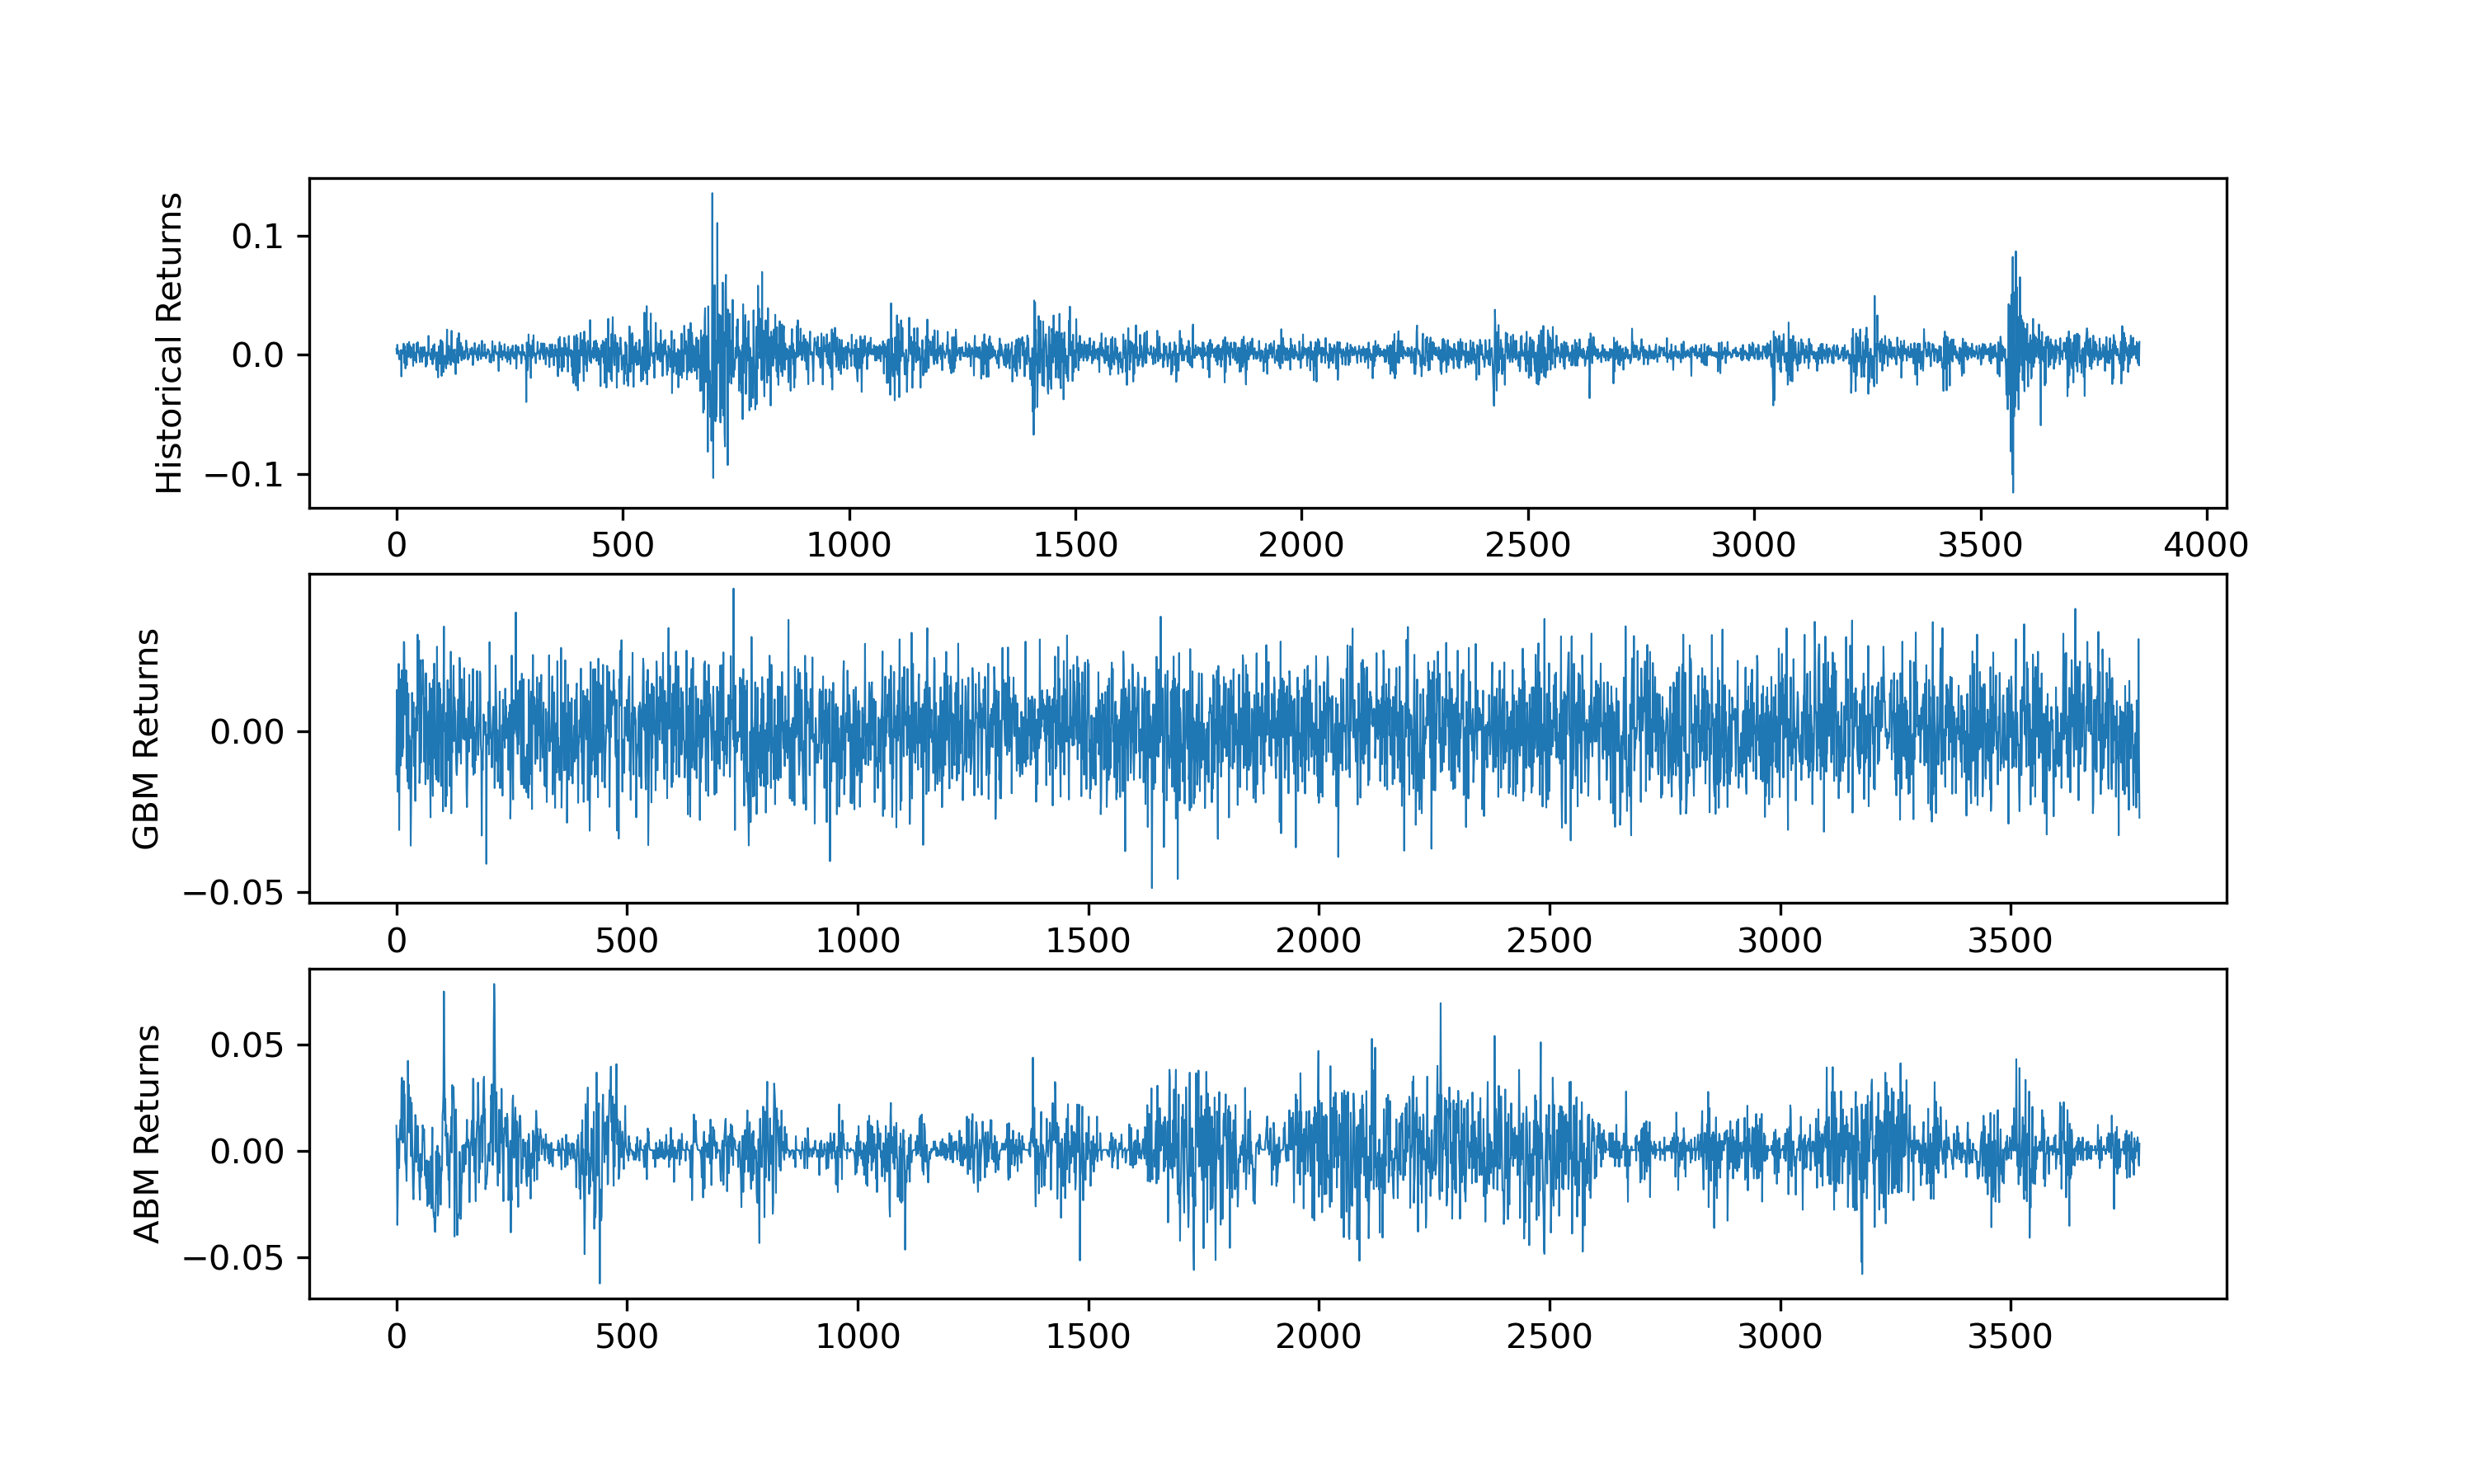
\includegraphics[scale=0.6, trim=0cm 1.5cm 0cm 1cm]{returns.png} %trim={<left> <lower> <right> <upper>}
\end{center}
\caption{Returns}
\label{fig:returns}
\end{figure}



















\section{Discussion and Conclusion}

\begin{itemize}
\item Limitations and possible future direction.
\end{itemize}

























\begin{thebibliography}{99} 

\bibitem{lux}
Alfarano, S. and T. Lux. 2007. A Noise Trader Model as a Generator of Apparent Financial Power Laws and Long Memory. {\em Macroeconomic Dynamics}, 11, 80-101.

\bibitem{tsay}
Tsay, R. 2013. {\em An Introduction to Analysis of Financial Data with R.} Wiley. 

\end{thebibliography}


\end{document}
